\documentclass[11pt]{article}

\usepackage[left=2cm,right=2cm,top=2cm,bottom=2cm]{geometry} 

\usepackage[utf8]{inputenc}   % otra alternativa para los caracteres acentuados y la "ñ"
\usepackage[           spanish % para poder usar el español
                      ,es-tabla % para los captions de las tablas
                       ]{babel}   
\decimalpoint %para usar el punto decimal en vez de coma para los números con decimales

%\usepackage{beton}
%\usepackage[T1]{fontenc}

\usepackage{parskip}
\usepackage{xcolor}

\usepackage{caption}

\usepackage{fancyvrb}

\usepackage{enumerate} % paquete para poder personalizar fácilmente la apariencia de las listas enumerativas

\usepackage{graphicx} % figuras
%\usepackage{subfigure} % subfiguras
\usepackage{subcaption}

\usepackage{amsfonts}
\usepackage{amsmath}

\usepackage[formats]{listings}
\lstdefineformat{R}{~=\( \sim \)}
\lstset{basicstyle=\ttfamily,format=R}

\definecolor{gris}{RGB}{220,220,220}
	
\usepackage{float} % para controlar la situación de los entornos flotantes

\restylefloat{figure}
\restylefloat{table} 
\setlength{\parindent}{0mm}


\usepackage[bookmarks=true,
            bookmarksnumbered=false, % true means bookmarks in 
                                     % left window are numbered
            bookmarksopen=false,     % true means only level 1
                                     % are displayed.
            colorlinks=true,
            allcolors=blue,
            urlcolor=blue]{hyperref}
\definecolor{webblue}{rgb}{0, 0, 0.5}  % less intense blue


\title{\Huge Ataques Man-in-the-Middle \vspace{10mm}}

\author{\Large Grupo 1: \vspace{10mm} \\
	\Large David Cabezas Berrido \vspace{5mm} \\ 
  \Large dxabezas@correo.ugr.es \vspace{10mm} \\
  \Large Patricia Córdoba Hidalgo \vspace{5mm} \\ 
	\Large patriciacorhid@correo.ugr.es \vspace{10mm}}

\begin{document}
\maketitle
\vfill
\begin{flushleft}
{\Large Horas dedicadas al desarrollo del trabajo: 11}
\end{flushleft}
\vspace{40mm}
~
\newpage
\tableofcontents
\newpage

\section{Simulación de ataque}

A continuación, mostramos una simulación de un ataque Man-in-the-Middle, seguiremos
\href{https://www.youtube.com/watch?v=fbXu8EX0hsI}{este tutorial}. 

Creamos una nueva red local: \texttt{vboxnet1}. En ella tendremos los siguientes hosts:
\begin{itemize}
	\item Máquina anfitriona: El atacante. Tiene Ubuntu 20.04.2 LTS.
	\item Cliente: Una de las víctimas del ataque.
	\item Servidor: La otra víctima. Tiene el servicio de Apache2 básico, por el que sirve un \texttt{index.html} con el mensaje
	``Hellow World!''.
\end{itemize}

En la siguiente tabla podemos ver las direcciones (IP y MAC) de cada uno de los hosts.

\begin{table}[H]
	\centering
	\begin{tabular}{|c|c|c|}
		\hline
		\textbf{Host} & \textbf{IP}  & \textbf{MAC}      \\ \hline
		Atacante      & 192.168.57.1 & 0a:00:27:00:00:01 \\ \hline
		Cliente       & 192.168.57.3 & 08:00:27:01:3a:c8 \\ \hline
		Servidor      & 192.168.57.4 & 08:00:27:6c:b7:f2 \\ \hline
	\end{tabular}
	\caption{Direcciones de las máquinas en la red \texttt{vboxnet1}.}
	\label{tab:info-hosts}
\end{table}

\subsubsection*{Herramientas}

Instalamos las siguientes herramientas en la máquina atacante.

Debemos instalar \href{https://www.ettercap-project.org}{Ettercap}, un paquete con utilidades para este tipo de ataques.
Podemos hacerlo desde Ubuntu Software.

Para monitorizar el ataque utilizaremos Wireshark. También usaremos \texttt{urlsnarf} para husmear el tráfico HTTP entre las víctimas. Esta
herramienta muestra las las peticiones HTTP que se realizan. Para descargarla, utilizamos el comando \verb^sudo apt install dsniff^.

\subsubsection*{Ataque}

El primer paso es activar la redirección de paquetes en la máquina atacante. De otro modo, las víctimas no podrían comunicarse entre sí, ya
que los paquetes serían interceptados por el atacante, y se percatarían rápidamente del ataque. Podemos lograr esto ejecutando la orden
\verb|sysctl -w net.ipv4.ip_forward=1|, o escribiendo el valor 1 en el fichero \texttt{/proc/sys/net/ipv4/ip\_forward}.

\begin{figure}[H]
	\centering
	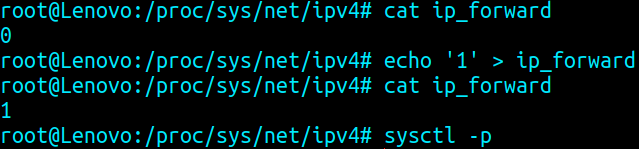
\includegraphics[width=110mm]{images/ip_forward}
	\caption{Activamos la redirección de paquetes escribiendo un 1 en el fichero \texttt{/proc/sys/net/ipv4/ip\_forward}.}
	\label{fig:ip_forward}
\end{figure}

Tras esto ejecutamos el comando \verb|sysctl -p| para hacer efectivos los cambios recién realizados.

Seguidamente, lanzamos Ettercap en el atacante, especificando el nombre de la interfaz de red que queremos atacar: \texttt{vboxnet1}.

\begin{figure}[H]
	\centering
	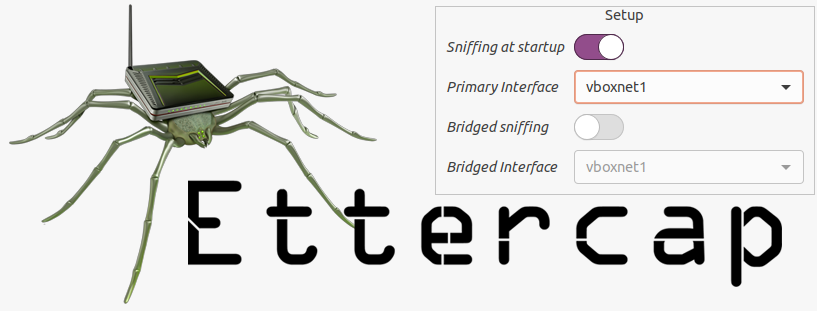
\includegraphics[width=140mm]{images/ettercap-start}
	\caption{Pantalla de inicio de Ettercap. Seleccionamos la red \texttt{vboxnet1}.}
	\label{fig:ettercap-start}
\end{figure}

Al entrar, recibimos los siguientes mensajes en la parte inferior de la ventana.

\begin{Verbatim}[tabsize=4]
Listening on:
vboxnet1 -> 0A:00:27:00:00:01
	192.168.57.1/255.255.255.0
	fe80::800:27ff:fe00:1/64

SSL dissection needs a valid 'redir_command_on' script in the etter.conf file
Ettercap might not work correctly. /proc/sys/net/ipv6/conf/all/use_tempaddr is not set to 0.
Ettercap might not work correctly. /proc/sys/net/ipv6/conf/vboxnet1/use_tempaddr is not set to 0.
Privileges dropped to EUID 65534 EGID 65534...

34 plugins
42 protocol dissectors
57 ports monitored
24609 mac vendor fingerprint
1766 tcp OS fingerprint
2182 known services
Lua: no scripts were specified, not starting up!
Starting Unified sniffing...
\end{Verbatim}

Podemos detener y reanudar el sniffing (husmeo) pulsando el botón de stop/play en la esquina
 superior izquierda. Este comienza activado.
 
Pulsamos en el botón \textit{Scan for hosts}, la lupa que se encuentra en la esquina superior izquierda, para buscar los host conectados a dicha interfaz. Al hacer esto nos aparece el siguiente mensaje en la parte inferior de la ventana:

\begin{Verbatim}[tabsize=4]
Randomizing 255 hosts for scanning...
Scanning the whole netmask for 255 hosts...
3 hosts added to the hosts list...
\end{Verbatim}

Podemos ver los hosts encontrados pulsando en el botón que aparece a la derecha de la lupa, \textit{Hosts List}.

\begin{figure}[H]
	\centering
	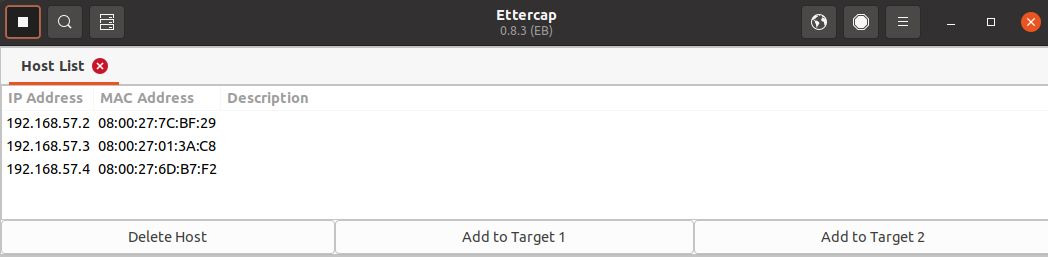
\includegraphics[width=140mm]{images/host-list}
	\caption{Lista de hosts conectados a la red \texttt{vboxnet1}.}
	\label{fig:host-list}
\end{figure}


Entre los hosts encontrados se encuentran nuestras dos víctimas. Seleccionamos el cliente, aquel con la dirección IP 192.168.57.3, y hacemos click en el botón \textit{Add to Target 1}. Análogamente seleccionamos el host con dirección IP 192.168.57.4 y hacemos click en el botón \textit{Add to Target 2}. Al hacer esto nos aparecen los siguientes mensages en la ventana inferior.

\begin{Verbatim}
Host 192.168.57.3 added to TARGET1
Host 192.168.57.4 added to TARGET2
\end{Verbatim}

La otra dirección que aparece, 192.168.57.2, corresponde al router.

Una vez seleccionadas nuestras víctimas procedemos a envenenar la caché de ARP, es decir, desde el atacante se enviarán paquetes a ambas víctimas para que estas lo identifiquen como la víctima contraria. Para ello pulsamos el botón de \textit{MITM Menu}, aquel con el logo del globo terráqueo situado en la esquina superior derecha, y seleccionamos la opción \textit{ARP poisoning}. 

\begin{figure}[H]
	\centering
	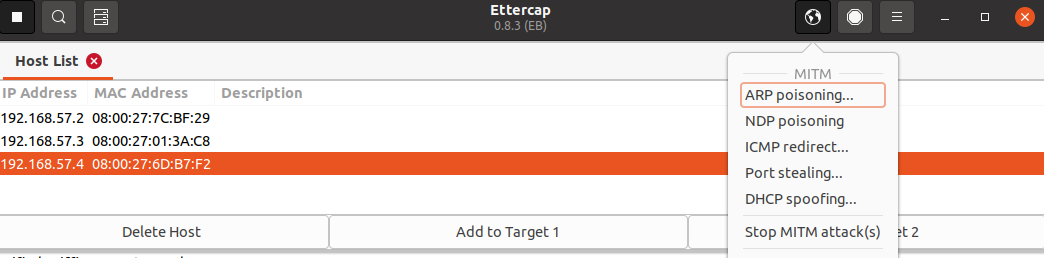
\includegraphics[width=140mm]{images/ettercap-mitm-arp-poisoning}
	\caption{Pulsamos en el botón \textit{MITM Menu}.}
	\label{fig:host-list}
\end{figure}

Nos aparece en una pantalla emergente con parámetros opcionales de esta funcionalidad. Marcamos el parámetro \textit{Sniff remote connections}.

\begin{figure}[H]
	\centering
	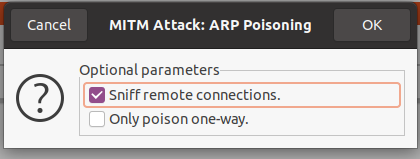
\includegraphics[width=90mm]{images/ettercap-arp-poisoning}
	\caption{Ventana emergente con las opciones de \textit{ARP poisoning}.}
	\label{fig:host-list}
\end{figure}

Obtenemos el siguiente mensage en la parte inferior de la ventana.

\begin{Verbatim}[tabsize=4]
ARP poisoning victims:

GROUP 1 : 192.168.57.3 08:00:27:01:3A:C8

GROUP 2 : 192.168.57.4 08:00:27:6D:B7:F2
\end{Verbatim}

\begin{figure}[H]
	\centering
	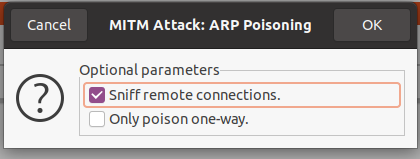
\includegraphics[width=90mm]{images/ettercap-arp-poisoning}
	\caption{Ventana emergente con las opciones de \textit{ARP poisoning}.}
	\label{fig:host-list}
\end{figure}

Abrimos Wireshark y capturamos los paquetes de la interfaz \texttt{vboxnet1}. Podemos observar que se envían varios paquetes desde 0a:00:27:00:00:01, el atacante, a ambas víctimas. Por ejemplo, si nos fijamos en el primer paquete capturado podemos comprobar que es un paquete del atacante al cliente. Este paquete informa al cliente de que la dirección IP 192.168.57.4 se encuentra en la dirección MAC del atacante, cuando realmente esa dirección IP pertenece al servidor. Análogamente en el segundo paquete observamos como el atacante informa al servidor de que la dirección IP del cliente, 192.168.57.3, se encuentra en la dirección física del atacante.

Por tanto, el atacante ha conseguido que ambas víctimas le identifiquen como la contraria, por lo que todo el tráfico que circule entre ambas máquinas pasará por este y será capaz de husmearlo. Ha envenenado la caché de ARP.

\begin{figure}[H]
	\centering
	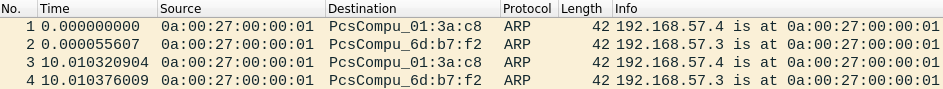
\includegraphics[width=140mm]{images/atack1/wireshark-arp}
	\caption{ARP poisoning. El atacante envía paquetes a sus víctimas con una identificación falsa.}
	\label{fig:wireshark-arp}
\end{figure}

Seguidamente, lanzamos \texttt{urlsnarf} en el atacante, indicando la interfaz de red con la opción \texttt{-i}. Esto nos permitirá
conocer las peticiones HTTP que se realicen entre el cliente y el servidor.

\subsubsection*{Análisis del tráfico}

El ataque ya está montado. Ahora hacemos CURL desde el cliente al servidor (\verb|curl http://192.168.57.4|).
Observamos la siguiente secuencia de intercambios en Wireshark.

\begin{figure}[H]
	\centering
	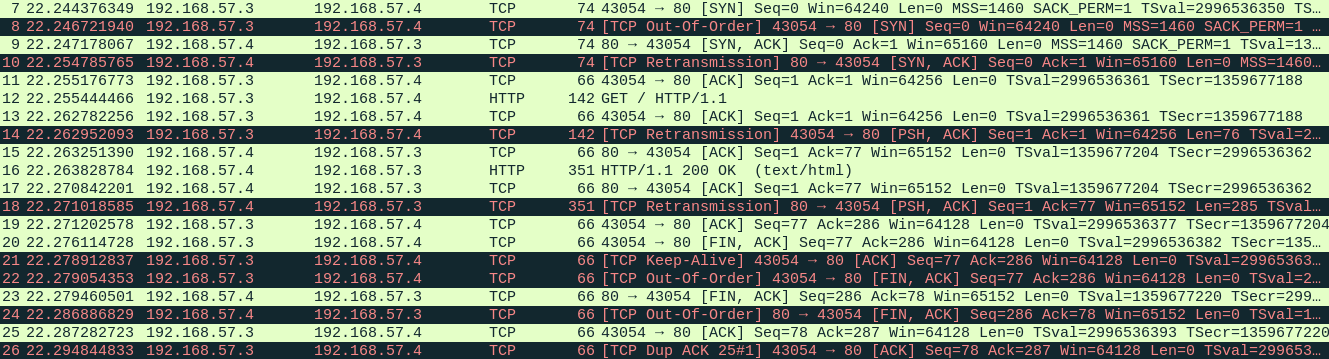
\includegraphics[width=170mm]{images/atack1/request}
	\caption{Comunicaciones capturadas mientras se realiza la petición.}
	\label{fig:request}
\end{figure}

Lo primero que nos llama la atención es la cantidad de paquetes \emph{Bad TCP}, que aparecen en negro y najanja. Esto
no es ningún fallo. Debido a que el atacante está actuando de intermediario, se realizan más intercambios de los esperados
entre las máquinas. A la hora de comprobar que la comunicación es correcta, Wireshark también piensa que el atacante es
una de las víctimas, de modo que la secuencia de paquetes que registra le confunde y piensa que se deben a errores en TCP. En 
seguida mostraremos ejemplos que reflejen esto.

Al analizar cualquiera de estos paquetes, tanto los relativos a la comunicación TCP (3-Way Handshake y cierre) como las peticiones y
respuestas HTTP, descubrimos que en ningún momento el cliente y el servidor consiguen comunicar directamente. A pesar de lo que aparece
en los campos IP origen e IP destino (tercera y cuarta columna), la dirección física de la máquina atacante aparece implicada
en cada transmisión. Observamos ésto analizando los paquetes 7 y 8, correspondientes a SYN. Podemos consultar las direcciones físicas en
la tabla \ref{tab:info-hosts}.

\begin{figure}[H]
	\centering
	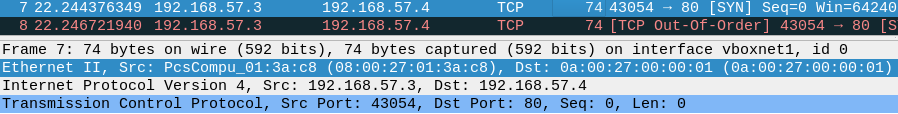
\includegraphics[width=160mm]{images/atack1/syn-client-atacker}
	\caption{Las direcciones IP y física de origen corresponden al cliente; y la dirección IP de destino es la del servidor. Sin embargo,
	la dirección física de destino realmente corresponde a la máquina atacante, que es la que realmente recibe el paquete. Esto se debe
	a un fallo en la caché de ARP del cliente, creado por el atacante. En nuestro caso, el paquete se reenvía a su verdadero destino,
	ya que activamos la redirección de paquetes, pero el atacante tiene la oportunidad de conocer el contenido.}
	\label{fig:syn-client-atacker}
\end{figure}

\begin{figure}[H]
	\centering
	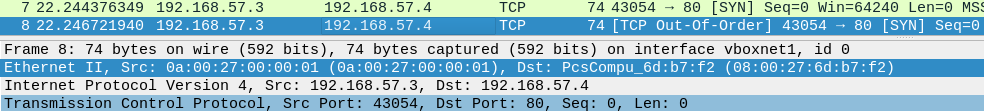
\includegraphics[width=160mm]{images/atack1/syn-atacker-server}
	\caption{El atacante reenvía el SYN al servidor y éste se piensa que procede del cliente debido a un error en la caché de ARP del servidor
		creado por el atacante. La dirección IP de origen es la del cliente y tanto la dirección IP como la dirección física de destino son las del servidor. La dirección física de origen es la del atacante. Puesto que Wiresharck interpreta que tanto el mensaje anterior como este son SYN que proceden de la misma IP y con la misma IP de destino piensa que se ha podido producir algún error durante el 3-Way Handshake. Por esto, señala este segundo paquete como \textit{Bad TCP} (Out-Of-Order).}
	\label{fig:syn-atacker-server}
\end{figure}

Analizamos ahora los paquetes correspondientes a la petición HTTP que se realiza de la máquina cliente al servidor. 

\begin{figure}[H]
	\centering
	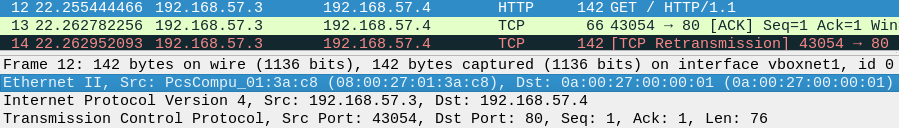
\includegraphics[width=160mm]{images/atack1/request-client-atacker}
	\caption{El cliente pretende mandar una petición HTTP al servidor. Podemos observar que la dirección IP y física de origen corresponden al cliente. La dirección IP de destino es la del servidor, pero la dirección física es la del atacante, luego realmente es al atacante al que se le manda la petición HTTP.}
	\label{fig:request-client-atacker}
\end{figure}

\begin{figure}[H]
	\centering
	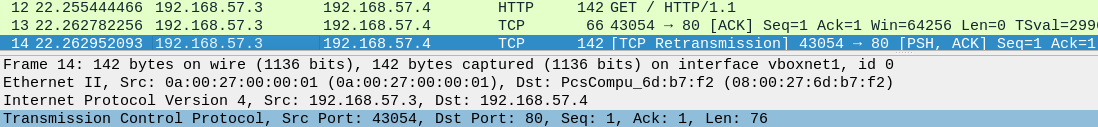
\includegraphics[width=160mm]{images/atack1/request-atacker-server}
	\caption{El atacante redirecciona la petición HTTP recibida al servidor. }
	\label{fig:request-atacker-server}
\end{figure}

\begin{figure}[H]
	\centering
	\begin{subfigure}{0.45\textwidth}
		\centering
		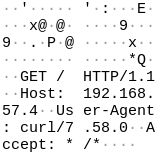
\includegraphics[width=30mm]{images/atack1/client-atacker}
		\captionsetup{width=0.5\linewidth}
		\caption{Contenido del paquete del cliente al atacante.}
	\end{subfigure}
	\hspace{-20mm}
	\begin{subfigure}{0.45\textwidth}
		\centering
		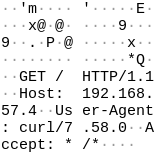
\includegraphics[width=30mm]{images/atack1/atacker-server}
		\captionsetup{width=0.5\linewidth}
		\caption{Contenido del paquete del atacante al servidor.}
	\end{subfigure}
	\caption{En el contenido del paquete podemos ver la petición HTTP mandada.}
\end{figure}

Del mismo modo, podemos analizar los paquetes de respuesta de la petición del servidor al cliente.

\begin{figure}[H]
	\centering
	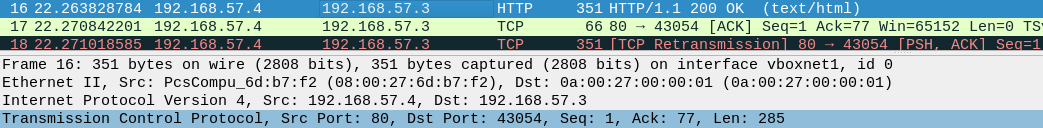
\includegraphics[width=160mm]{images/atack1/response-server-atacker}
	\caption{Como ocurre en el resto de paquetes, el servidor manda los paquetes cuya dirección IP de destino es el cliente a la dirección física del atacante. Así, el atacante puede husmear el contenido de los paquetes.}
	\label{fig:response-server-atacker}
\end{figure}

\begin{figure}[H]
	\centering
	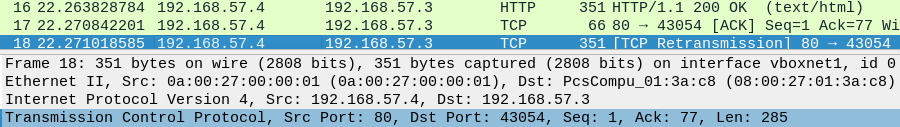
\includegraphics[width=160mm]{images/atack1/response-atacker-client}
	\caption{El atacante redirecciona el paquete recibido (la respuesta de la petición HTTP) al cliente.}
	\label{fig:response-atacker-client}
\end{figure}

\begin{figure}[H]
	\centering
	\begin{subfigure}{0.45\textwidth}
		\centering
		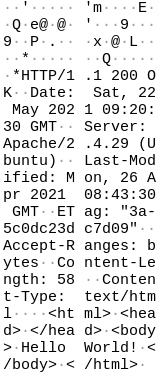
\includegraphics[width=30mm]{images/atack1/server-atacker}
		\captionsetup{width=0.5\linewidth}
		\caption{Contenido del paquete del servidor al atacante.}
	\end{subfigure}
	\hspace{-20mm}
	\begin{subfigure}{0.45\textwidth}
		\centering
		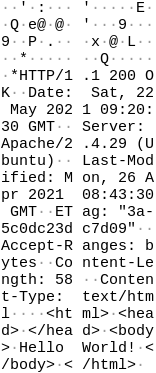
\includegraphics[width=30mm]{images/atack1/atacker-client}
		\captionsetup{width=0.5\linewidth}
		\caption{Contenido del paquete del atacante al cliente.}
	\end{subfigure}
	\caption{En el contenido del paquete podemos ver la respuesta de la petición HTTP mandada.}
\end{figure}

Además, \texttt{urlsnarf} registra cada petición HTTP que se haga entre las víctimas. Aparece una entrada por cada petición.

\begin{figure}[H]
	\centering
	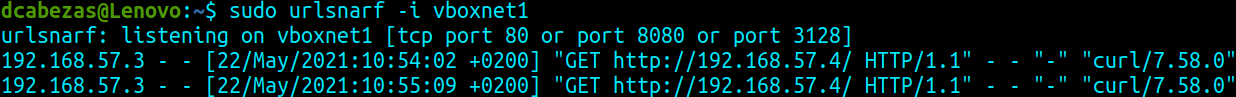
\includegraphics[width=160mm]{images/atack1/urlsnarf}
	\caption{Aparece una entrada por cada petición HTTP entre las víctimas.}
	\label{fig:urlsnarf}
\end{figure}

\section{Bibliografía}

% https://www.garron.me/es/gnu-linux/habilitar-ip-forward-linux-ubuntu.html
% https://www.ettercap-project.org
% https://www.youtube.com/watch?v=fbXu8EX0hsI

\end{document}
